
\section{Case-studies}\label{sec:evalation}

We conduct a series of experiments to evaluate the effectiveness of the dynamic adaptation algorithm.
First we evaluate the ability of the algorithm to adapt to runtime changes and reach an optimal thread-count, by comparing the thread-count given by the adaptation algorithm to an optimal thread-count that can be derived from the observations in Section~\ref{sec:observations}.

To evaluate how close the adaptation algorithm comes to the performance of a theoretical optimum, we compare its effectiveness against a hypothesized oracle that always determines the most energy-efficient number of threads.
To investigate whether there are differences between our energy-optimising approach and a runtime-optimising approach, we similarly compare our solution to the runtime-based adaptation algorithm described by Gordon et~al.~\cite{sac-mtdynamic}.
We investigate whether the adaptation algorithm introduces significant energy overhead, and finally we measure how much energy the adaptation algorithm saves compared to multiple static approaches.

Both the energy-based and runtime-based dynamic adaptation algorithms, the benchmark scripts, and the benchmark results are publicly available on GitHub~\cite{repo-mt}.
The implementation of the thread-switching beehive system and adaptation algorithm in \sac{} are available on the \sac{} GitLab project~\cite{repo-sac}.

\subsection{Thread-management in Single assignment C}\label{sec:implementation-sac}

We hook into \sac{}'s beehive system, explained in Section~\ref{sac-par}, to control the number of threads of \sac{} programs dynamically.
Before sending a signal to the worker bees to start processing, the queen requests the recommended thread-count and decreases or increases the size of the hive by putting worker bees to sleep or waking up sleeping bees, respectively.
Since the actual thread-count is fixed, we selectively put bees to sleep through the use of a semaphore.
The side-effect-free nature of the parallel code enables the required workload redistributions through the queen bee without any potential impact on the semantics of the program.
Instead of \sac{}'s standard busy wait, we use a semaphore to ensures that the threads of sleeping bees incur no additional energy consumption, and are free to be used by other processes on the system.
The queen bee wakes sleeping bees sending a message to their semaphore, after which these bees enter the busy wait state again, waiting for the signal to start working.

\subsection{Energy overhead}\label{sec:evalation-overhead}

With our goal of minimizing the energy consumption of programs, it is crucial that the adaptation algorithm itself does not introduce a significant amount of energy overhead.
We measure the overhead introduced by the adaptation algorithm by applying it to a function with an empty body.
The measured sources of overhead include the starting and stopping of each energy measurement, and the re-computation of the suggested thread-count when ten energy measurements have been supplied.
The energy consumption and runtime overhead are measured by repeating this process one million times.
We find that on average the algorithm has an energy overhead of $48\mu{}J$ and a runtime overhead of $5\mu{}s$.
Considering that even a single $500 \times 500$ matrix multiplication consumes around half a Joule in the best case, we conclude that the adaptation algorithm does not introduce significant energy overhead.

While there might be additional effects of the adaptation that cause overhead, such as context switches or other operating system effects, we fail to identify experiments that would quantify these effects.
We study the overhead that stems from the adjustment process itself in a series of experiments where we look at an execution where the problem-size is being changed over time.

\subsection{Adaptation quality}\label{sec:evalation-adaptation}

Factors such as input data size often change during the execution of a program.
A prominent real-world example this is observed in the training process of Convolutional Neural Networks, where each layer of the network operates on differently sized arrays.
We have observed in Section~\ref{sec:observations} that these changes can cause changes to the optimal thread-count.
A key requirement for the adaptation algorithm is its ability to adjust to those changes during the runtime of programs.
The objective is to dynamically converge towards the optimal thread-count under changing workload behaviours and system configurations.
We evaluate the adaptation quality of the algorithm by gradually changing the input data size to the examples from Section~\ref{sec:observations}, and assessing how effectively the adaptation algorithm converges to the thread-count with minimal energy consumption.

\begin{figure}[t]
    \centering
    \begin{minipage}[c]{0.49\linewidth}
        \centering
        \captionsetup{width=0.9\linewidth}
        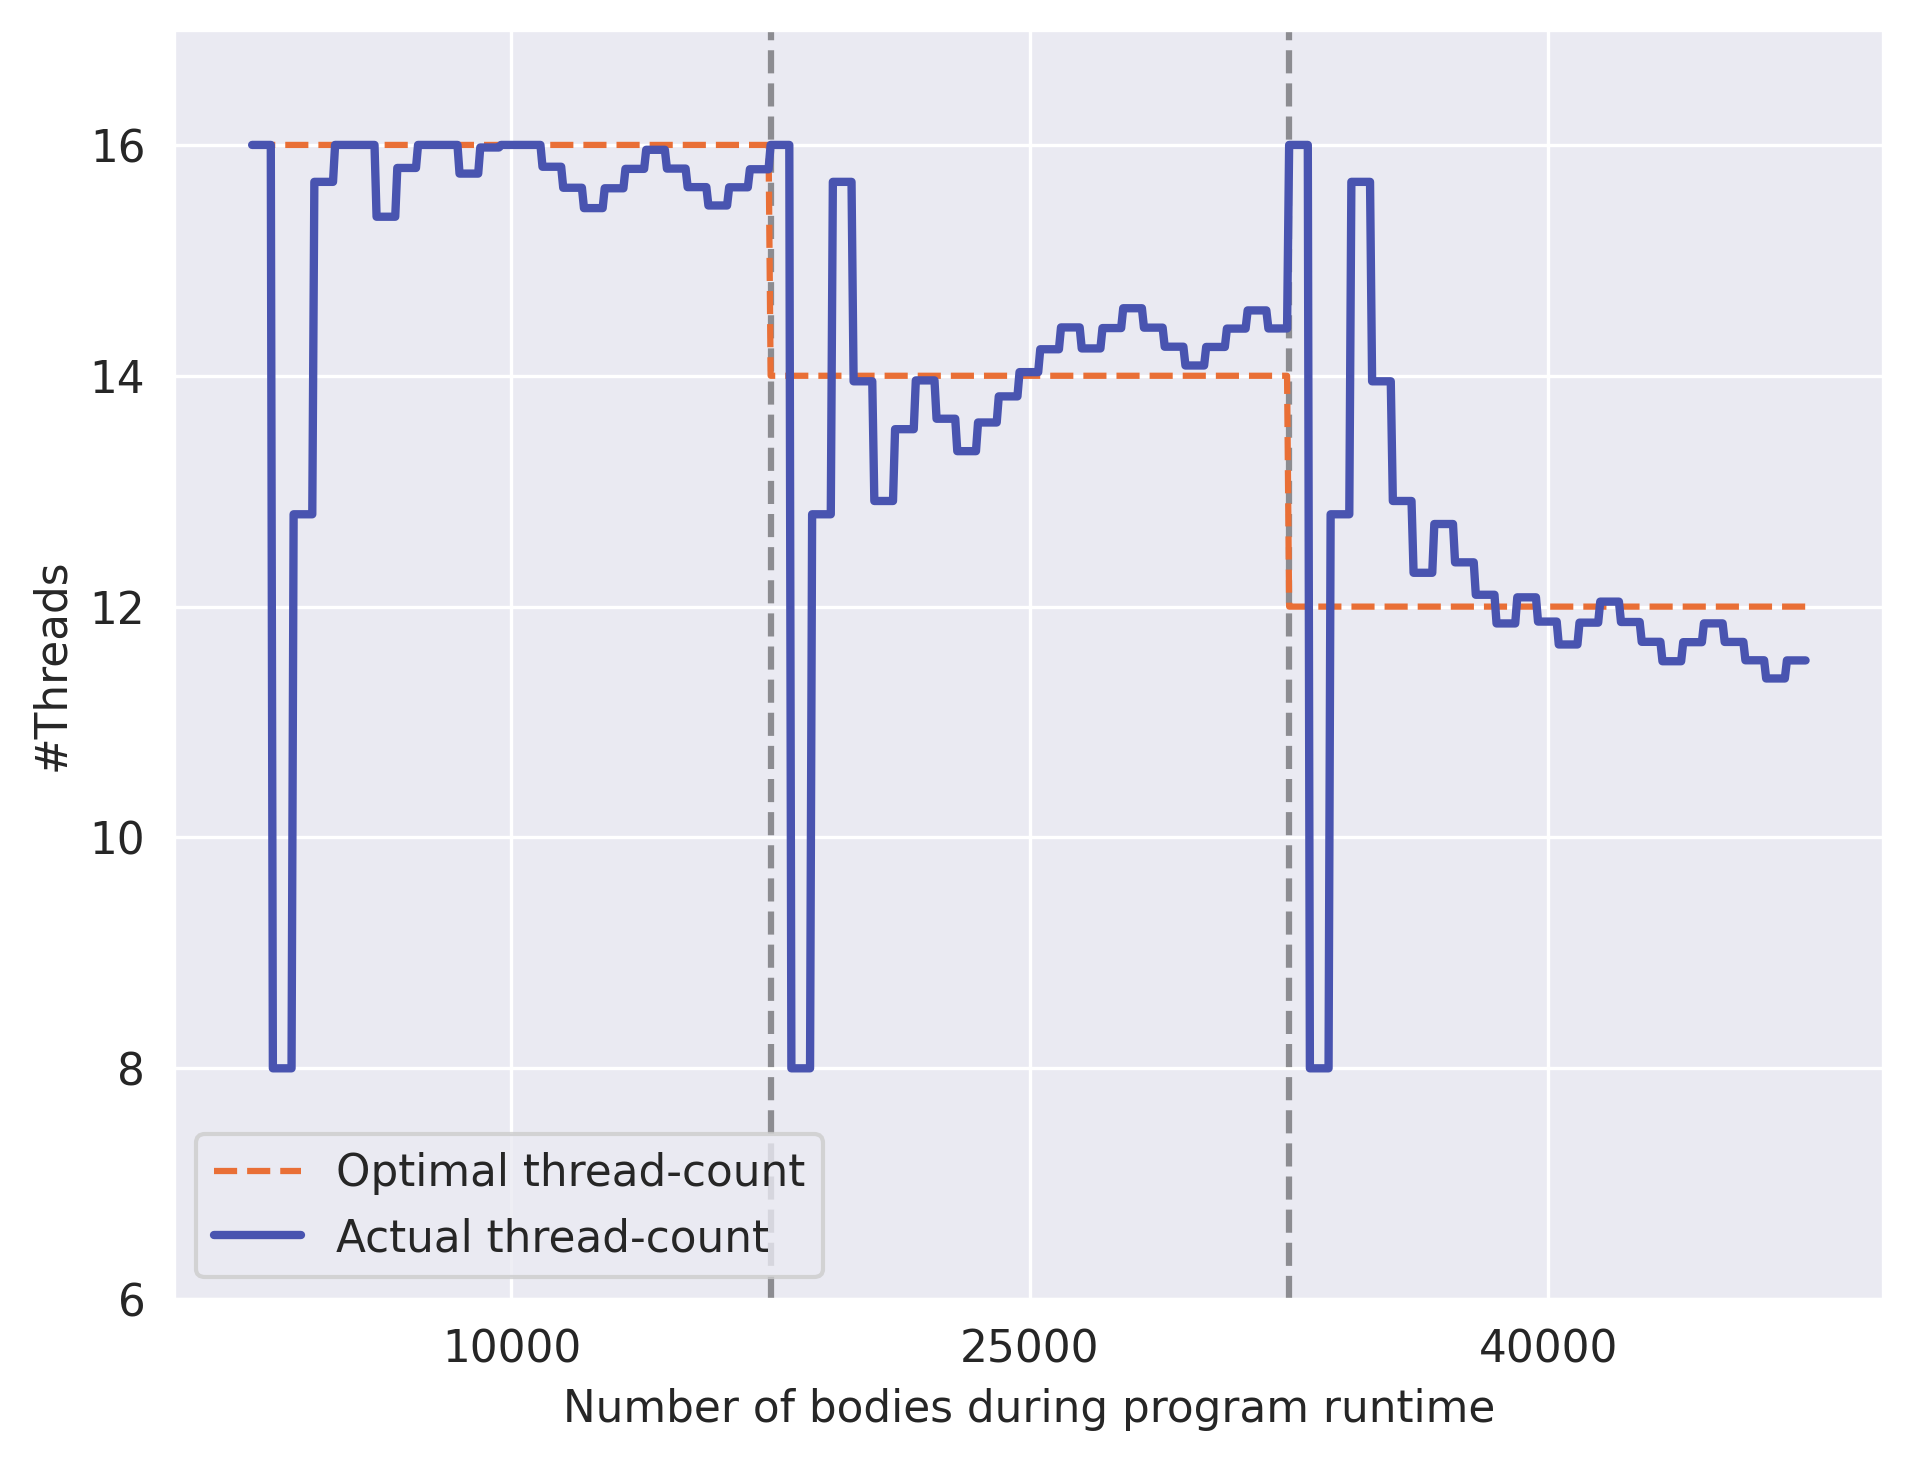
\includegraphics[width=\linewidth]{images/adapt_nbody.png}
        \caption{Adaptation quality on the \sac{} implementation of the N-body simulation.}
        \label{fig:adapt-nbody}
    \end{minipage}%
    \begin{minipage}[c]{0.49\linewidth}
        \centering
        \captionsetup{width=0.9\linewidth}
        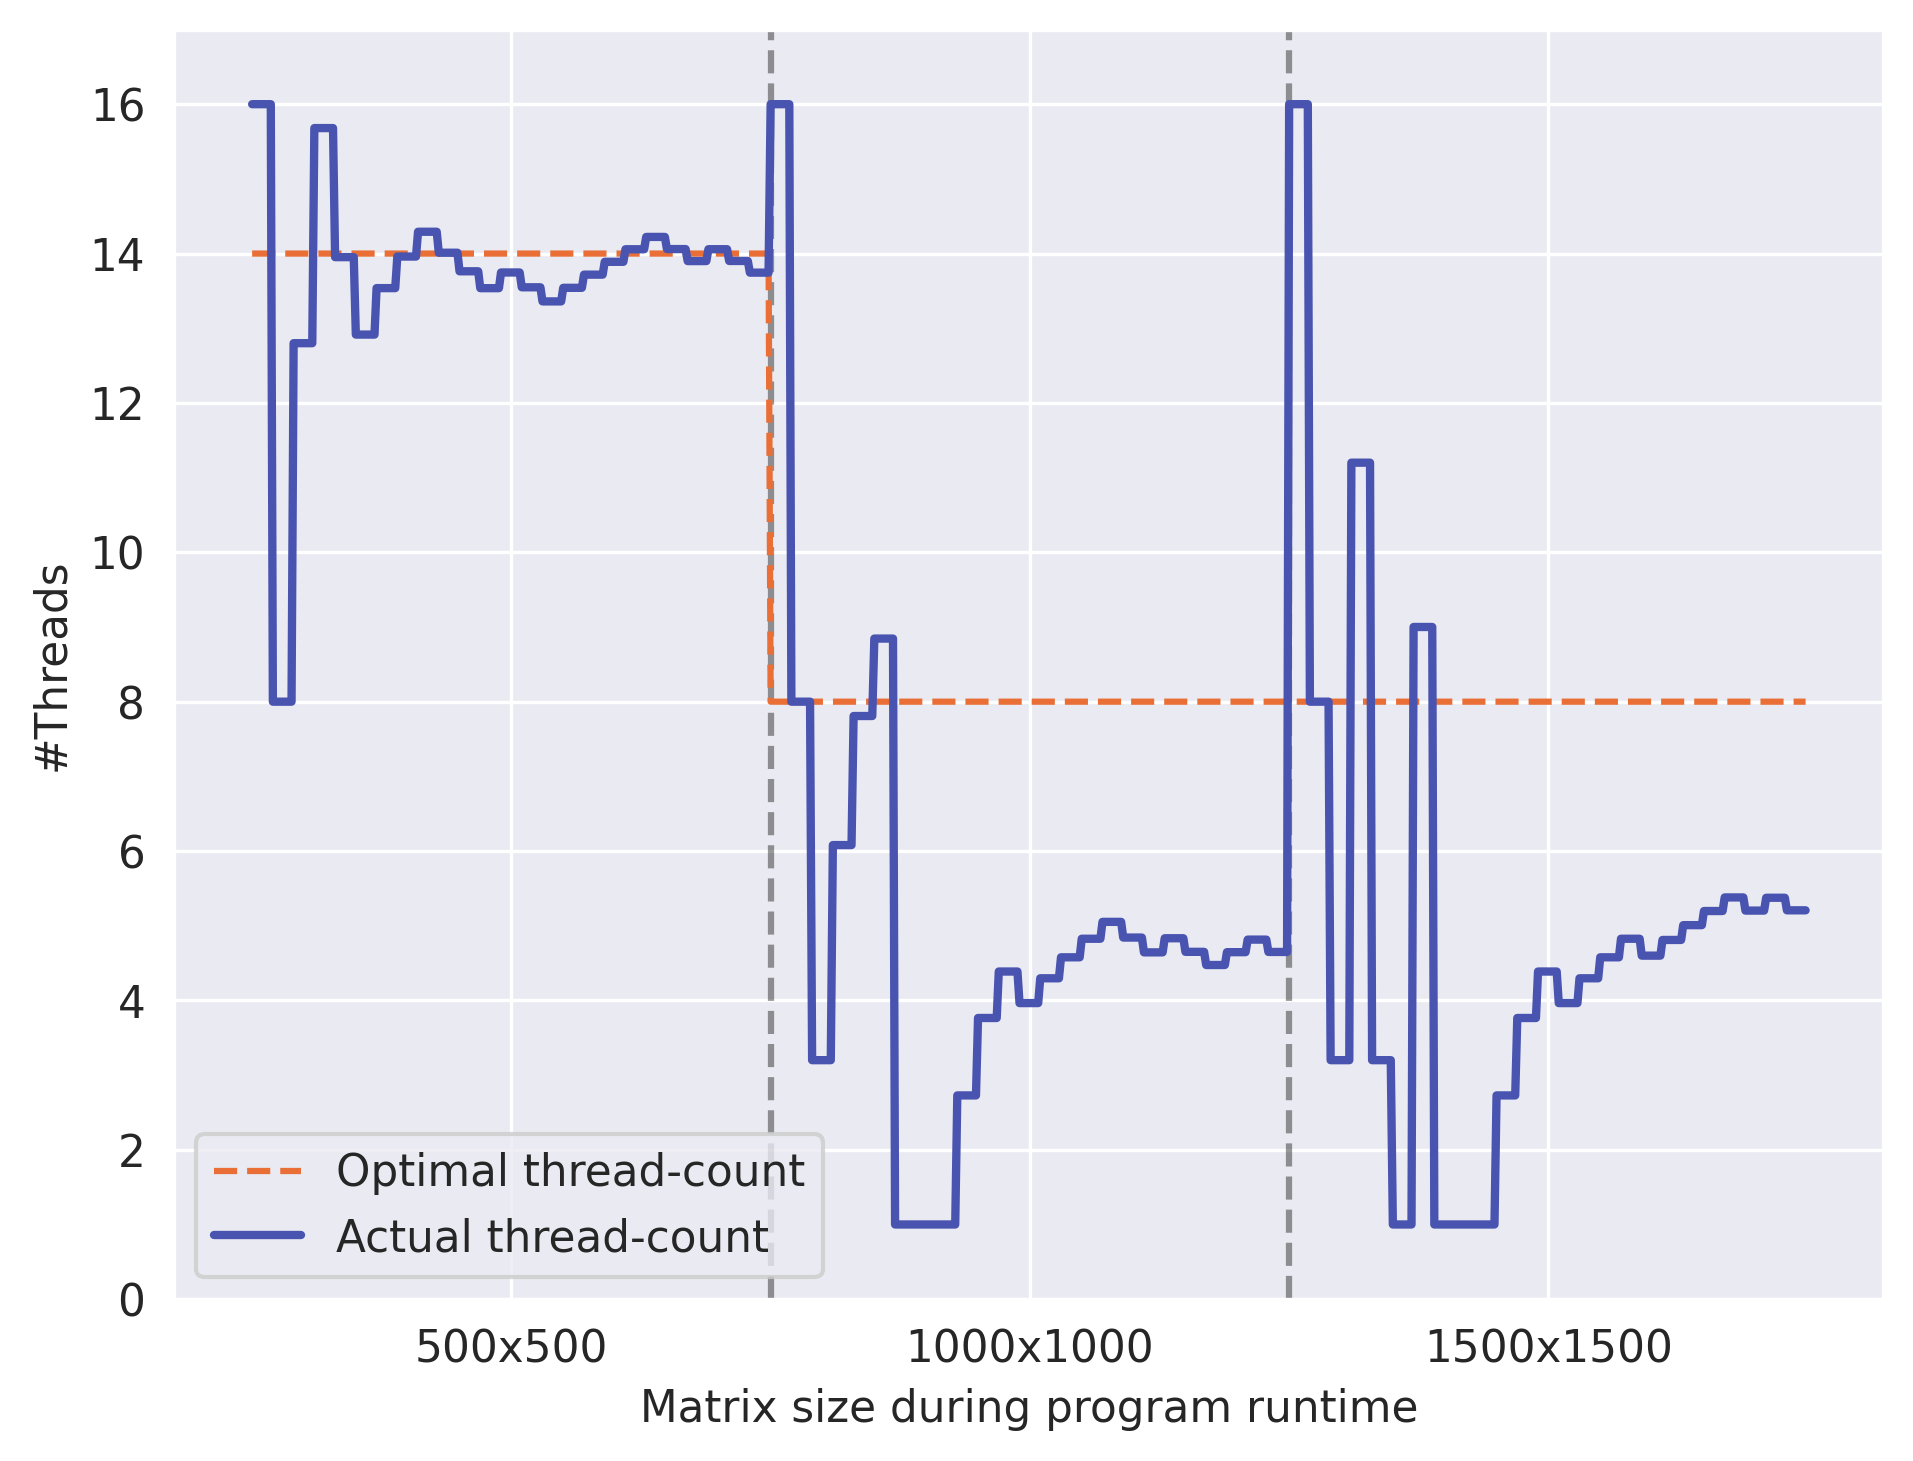
\includegraphics[width=\linewidth]{images/adapt_matmul.png}
        \caption{Adaptation quality on the \sac{} implementation of the matrix multiplication algorithm.}
        \label{fig:adapt-matmul}
    \end{minipage}%
\end{figure}

Figure~\ref{fig:adapt-nbody} shows the actual thread-count suggested by the adaptation algorithm across the runtime of the N-body simulation, alongside the optimum thread-count determined in Section~\ref{sec:observations}.
The x-axis represents the iterations of the program, where the input data size, denoted by the x-axis labels, changes at fixed intervals.
The orange dashed line shows the optimal thread-count derived from the observations in Section~\ref{sec:observations}, and the blue line shows the thread-count suggested by the adaptation algorithm.
The closer the suggested thread-count comes to the derived optimum, the better the adaptation quality of the algorithm.

In Figure~\ref{fig:adapt-nbody} we observe that the energy consumption plateaus when using eight or more threads.
Thread-counts between eight and sixteen threads are close in terms of energy-efficiency.
Even so, we see that the adaptation algorithm is able to find the optimum thread-count for the N-body simulation for each of the three input sizes.
For brevity we exclude the N-body simulation from the remaining benchmarks, as it provides a slightly better, but similar, level of performance compared to the nine-point stencil benchmark, and presents no further noteworthy results or insights.

The \sac{} implementation of the matrix multiplication algorithm presents an interesting challenge.
As discussed in Section~\ref{sec:observations}, choosing an effective thread pinning strategy is crucial to performance.
Whereas an interleaved pinning strategy is optimal when using eight or fewer threads, a contiguous strategy is more effective when using more than eight threads.
A drawback of our approach is that threads are disabled in a contiguous order, which results in a suboptimal pinning strategy for this benchmark.
In Figure~\ref{fig:adapt-matmul} we see that for $500 \times 500$ inputs we converge to the optimal thread-count at fourteen threads, even though the local optimum at eight threads only consumes slightly more energy.
However, for the other two input sizes the recommended thread-count around four threads, instead of eight.
This happens because the dynamic algorithm disables threads in a contiguous order, resulting in a poor thread pinning strategy.

\begin{figure}[t]
    \centering
    \begin{minipage}[c]{0.49\linewidth}
        \centering
        \captionsetup{width=0.9\linewidth}
        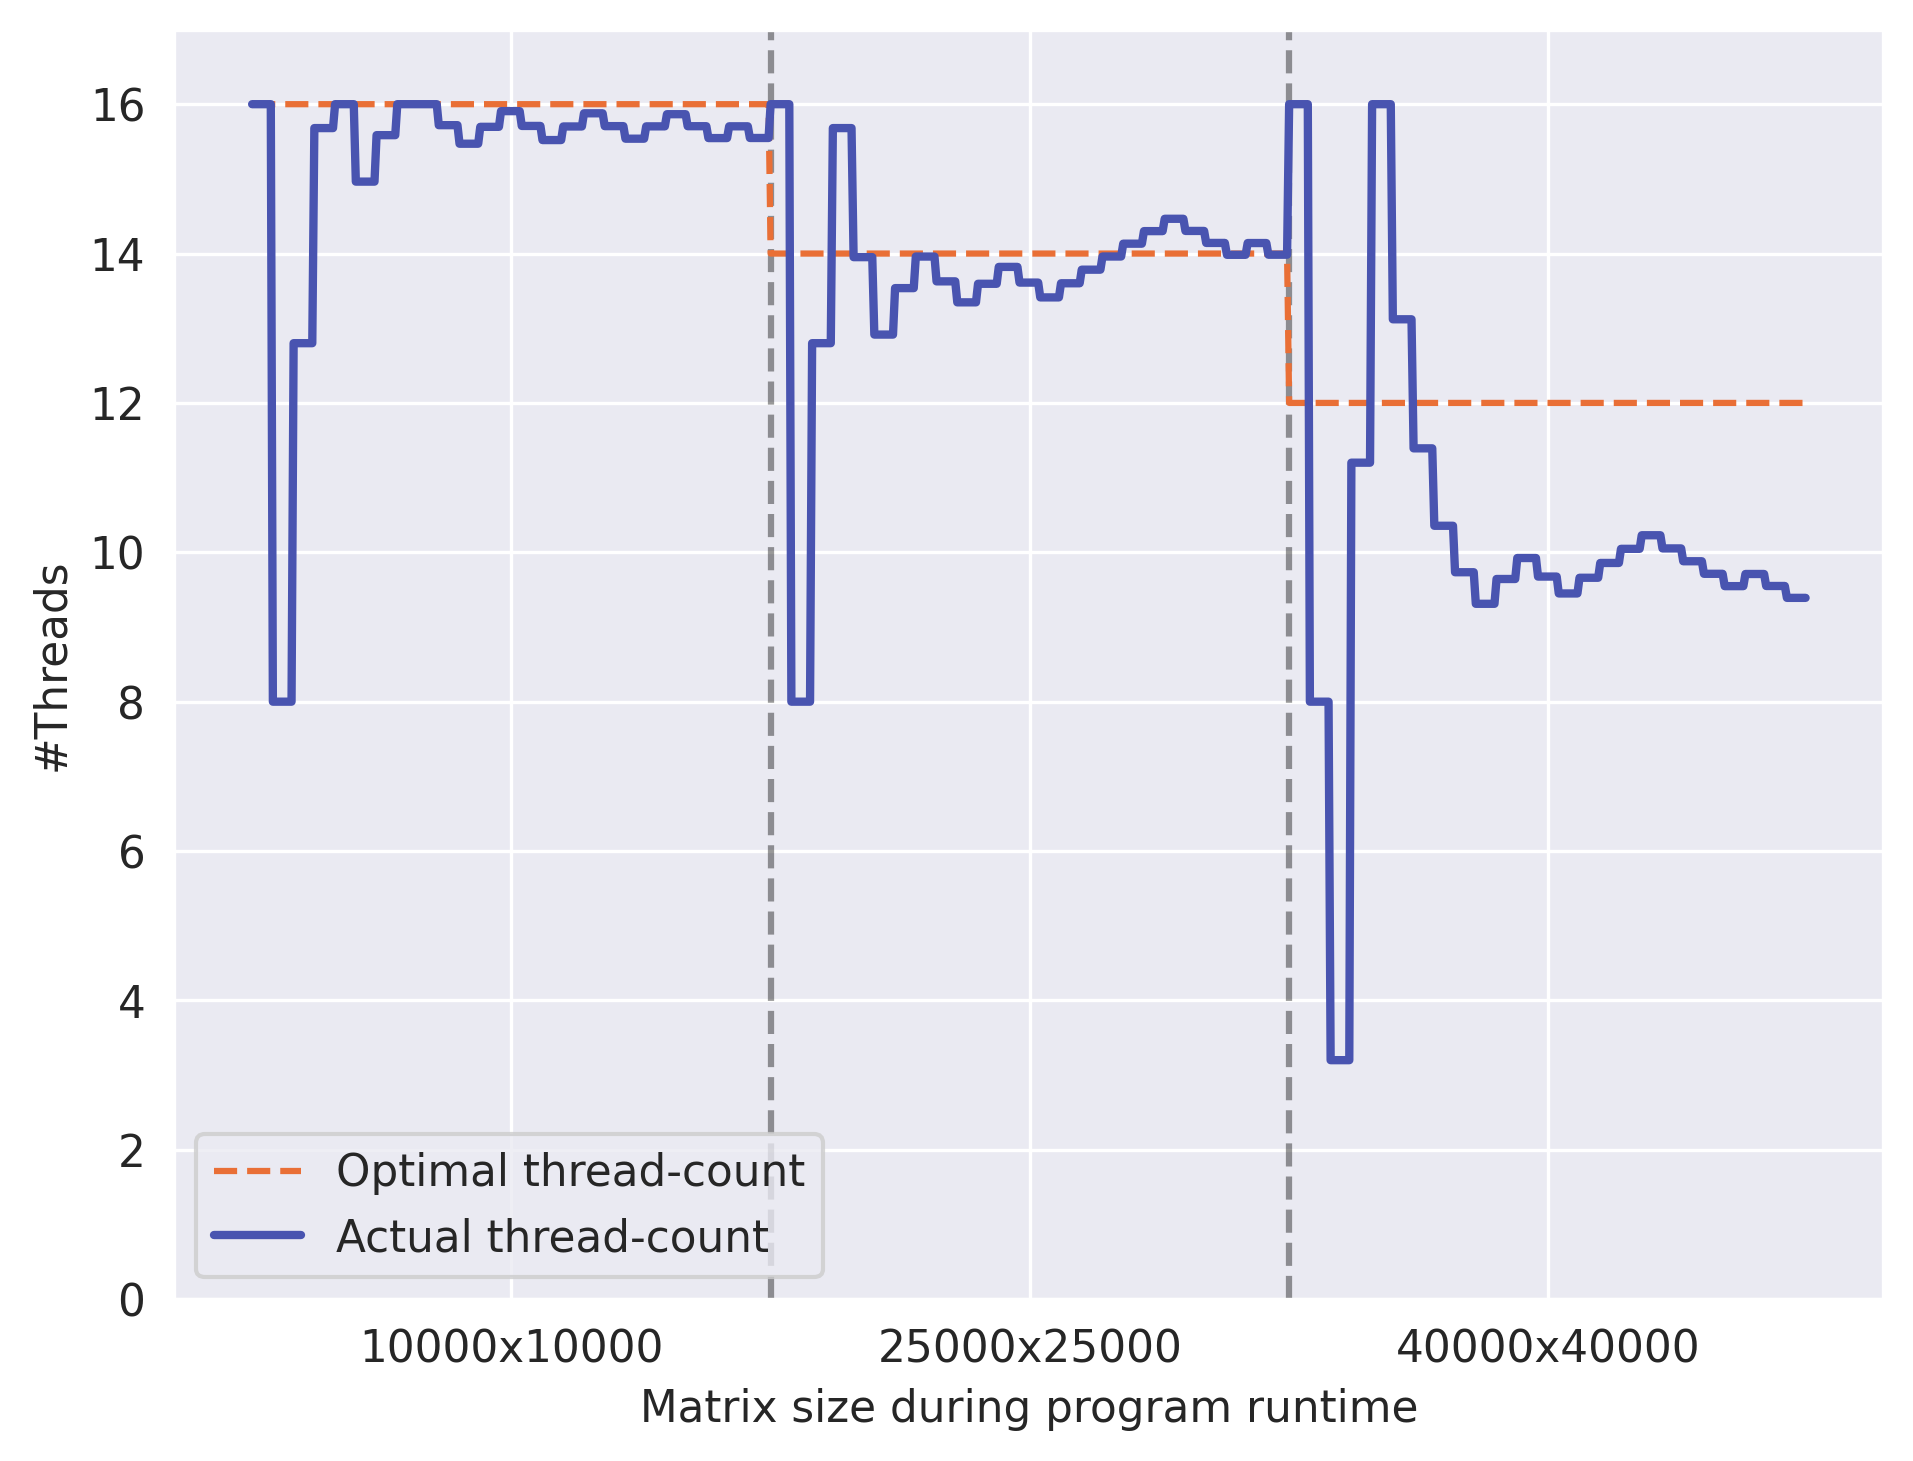
\includegraphics[width=\linewidth]{images/adapt_stencil.png}
        \caption{Adaptation quality on the \sac{} implementation of the nine-point stencil operation.}
        \label{fig:adapt-stencil}
    \end{minipage}%
    \begin{minipage}[c]{0.49\linewidth}
        \centering
        \captionsetup{width=0.9\linewidth}
        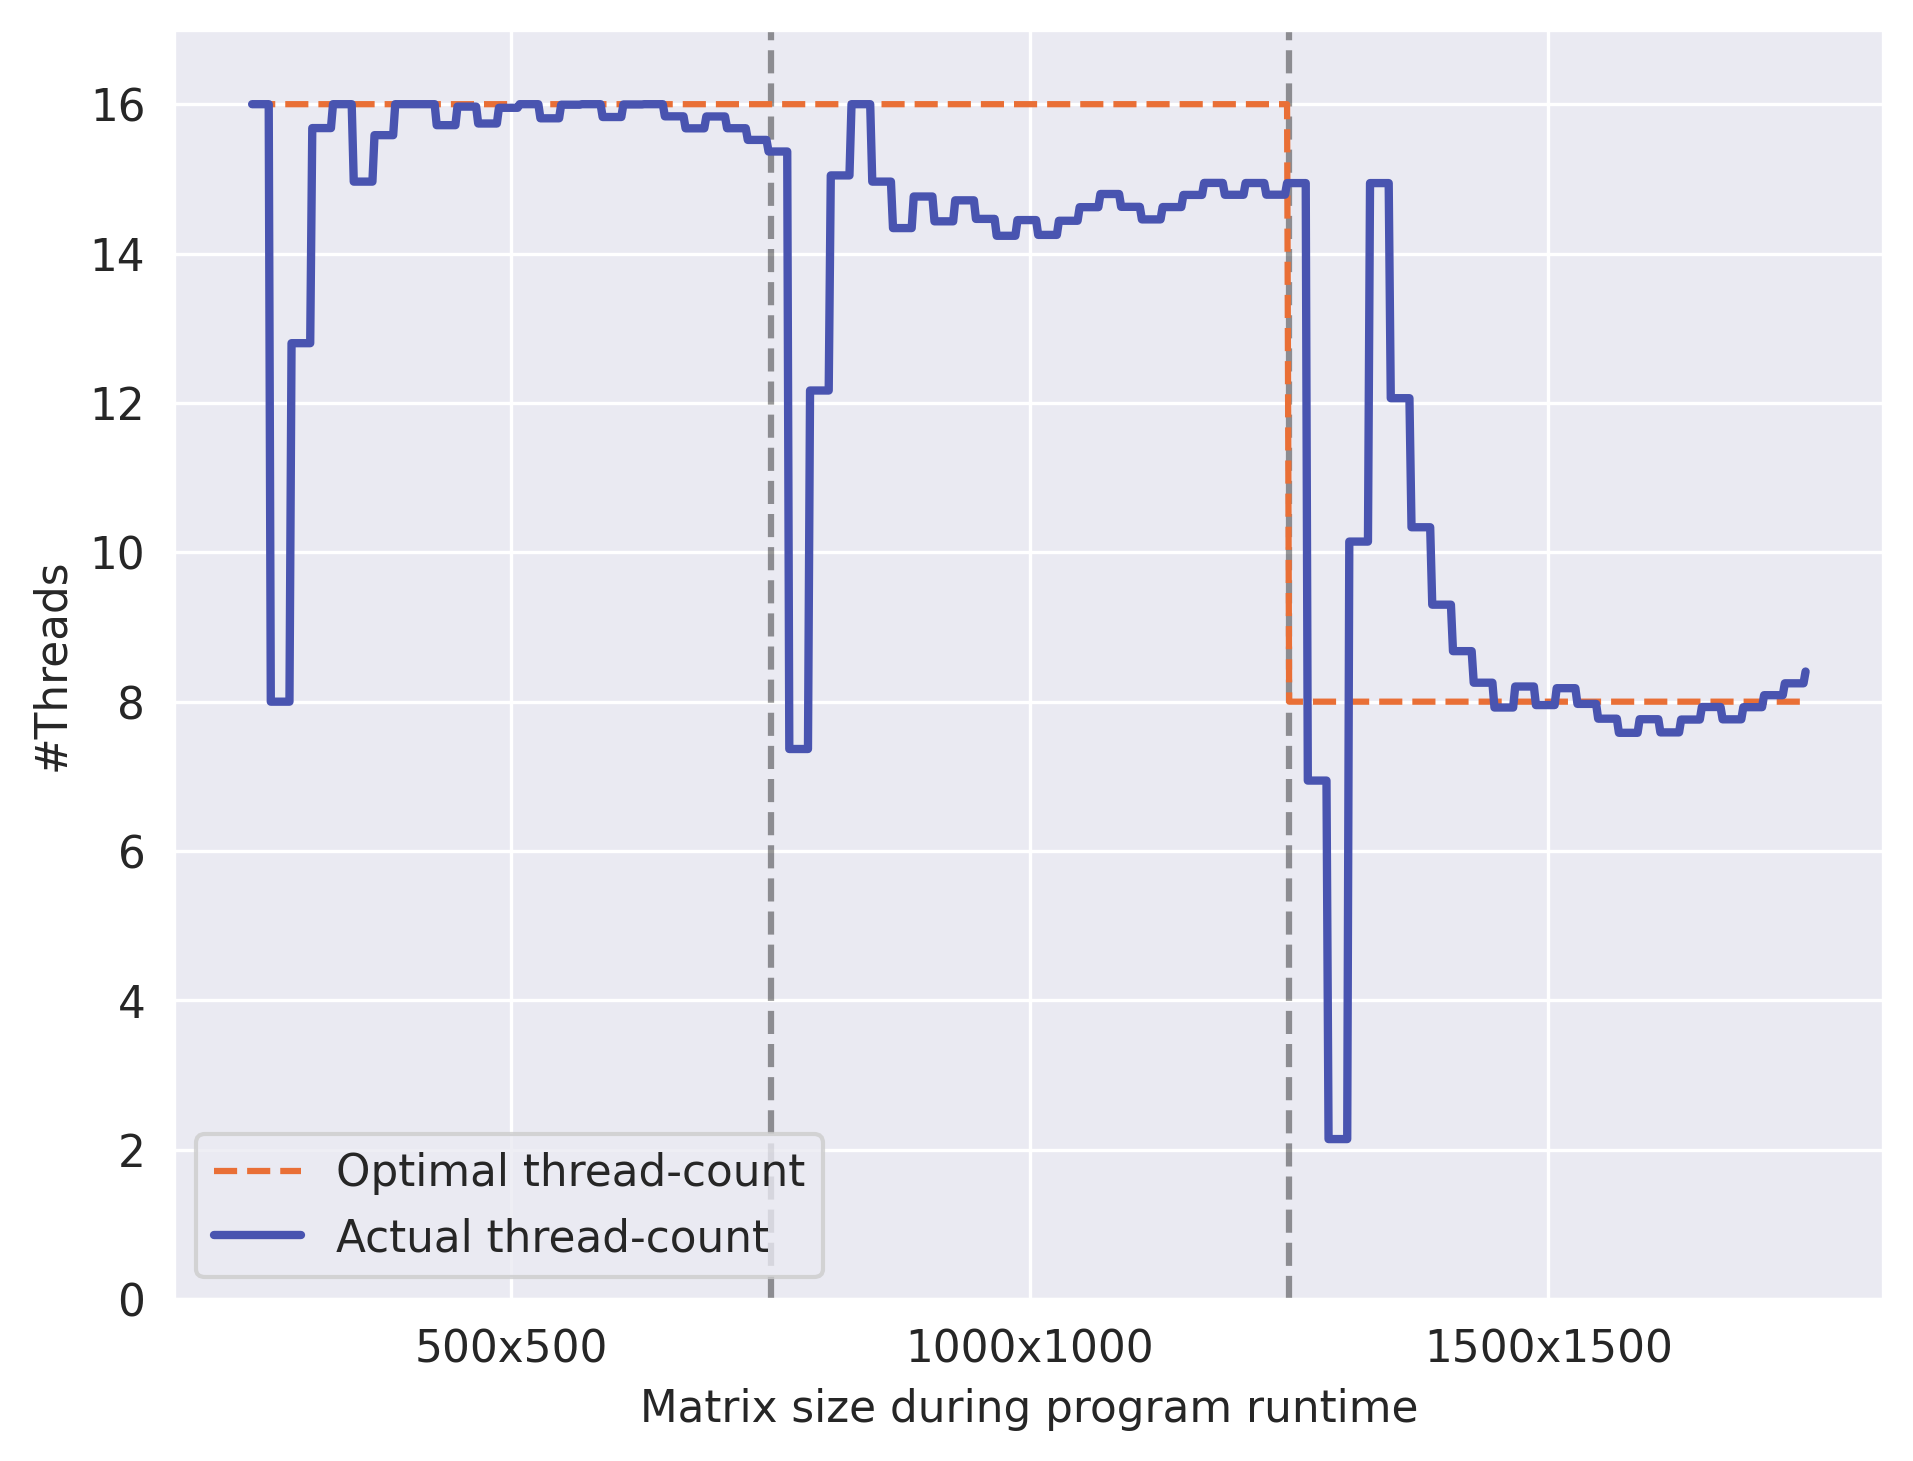
\includegraphics[width=\linewidth]{images/adapt_rust.png}
        \caption{Adaptation quality on the Rust implementation of the matrix multiplication algorithm.}
        \label{fig:adapt-rust}
    \end{minipage}%
\end{figure}

In Section~\ref{sec:observations} we observe for the nine-point stencil benchmark that as the input data size increases, the optimal thread-count gradually decreases.
Applying the adaptation algorithm we see in Figure~\ref{fig:adapt-stencil} that it is able to converge to the optimal thread-count in these cases.
Although for $40000 \times 40000$ inputs the algorithm suggests a thread-count of ten instead of twelve threads, Figure~\ref{fig:stencil3} shows that the energy consumption at these two thread-counts are within margin of error.

Figure~\ref{fig:adapt-rust} shows the adaptation quality for the Rust implementation.
The adaptation algorithm is able to quickly find the optimal thread-count after a change in the matrix size or system configuration.

These experiments show that the dynamic adaptation algorithm is capable of adequately adapting to runtime changes, except in outlier cases such as the $1500 \times 1500$ matrix multiplication in \sac{} where we do however find the local optimum given the suboptimal thread pinning strategy.
When a change in the energy consumption pattern occurs, the adaptation algorithm is able to convert to the optimal thread-count within a few thread-count adjustments.

\subsection{Comparison to oracle-based approach}\label{sec:evalation-oracle}

To further evaluate the effectiveness of the dynamic adaptation algorithm we compare its performance against a theoretical ``oracle'' approach.
This theoretical oracle knows which thread-count will result in the lowest energy consumption for the current implementation, workload behaviour, and hardware characteristics.
Although in general this level of foresight is unattainable without an analysis like the one in Section~\ref{sec:observations}, it provides a theoretical upper bound for the performance of the chosen benchmarks.
These optimums serve as the baseline to simulate the decision-making process of the oracle.
This oracle represents the best possible energy consumption, so any solution that closely approaches its performance can be considered highly effective.

\begin{table*}[ht]
    \centering
    \begin{subtable}{0.33\linewidth}
        \centering
        \begin{tabular}{ccc}\hline
            Input     & Energy & Runtime \\\hline
            $10000^2$ &    5\% &     4\% \\
            $25000^2$ &    5\% &     5\% \\
            $40000^2$ &   15\% &    33\% \\\hline
        \end{tabular}
        \caption{Nine-point stencil.}
        \label{tab:oracle-stencil}
    \end{subtable}%
    \begin{subtable}{0.33\linewidth}
        \centering
        \begin{tabular}{ccc}\hline
            Input    & Energy & Runtime \\\hline
            $ 500^2$ &    8\% &     8\% \\
            $1000^2$ &   46\% &    93\% \\
            $1500^2$ &   68\% &   100\% \\\hline
        \end{tabular}
        \caption{Matrix multiplication.}
        \label{tab:oracle-matmul}
    \end{subtable}%
    \begin{subtable}{0.33\linewidth}
        \centering
        \begin{tabular}{ccc}\hline
            Input    & Energy & Runtime \\\hline
            $ 500^2$ &    1\% &     1\% \\
            $1000^2$ &    1\% &     0\% \\
            $1500^2$ &   10\% &    16\% \\\hline
        \end{tabular}
        \caption{Rust implementation.}
        \label{tab:oracle-rust}
    \end{subtable}%
    \caption{Energy and runtime difference of the energy-based approach compared to the theoretical best performance of the oracle-based approach.}
    \label{fig:oracle}
\end{table*}

The comparison to the nine-point stencil operation is shown in Table~\ref{tab:oracle-stencil}.
It shows that, for $10000 \times 10000$ and $25000 \times 25000$ inputs, the dynamic approach provides a similar level of performance compared to the oracle, with only a 5\% increase in energy consumption.
However, for $40000 \times 40000$ inputs the energy consumption is increased by 15\% compared to the oracle.
In Figure~\ref{fig:adapt-stencil} we observed that for this input size the adaptation algorithm recommends ten threads, instead of the optimal thread-count of twelve threads.
Although this thread-count has a similar energy consumption compared to running at twelve threads, it does have significantly worse runtime, leading to a 33\% increase in runtime.
The decrease in energy-efficiency can be attributed to the additional energy cost introduced by the operating system, as well as the power required to keep the hardware operational (Section~\ref{sec:defining-energy}), which increases as the runtime increases.
Considering these additional energy requirements due to an increase in runtime, a 15\% increase in energy consumption compared to a 33\% increase in runtime seems reasonable.

Table~\ref{tab:oracle-matmul} shows how close the adaptive algorithm comes to the theoretical best performance on the matrix multiplication algorithm, provided by the oracle.
For $500 \times 500$ inputs we are within 8\% of the energy consumption and runtime of the oracle-based approach.
However, for the larger input sizes the performance deteriorates.
As discussed in Section~\ref{sec:evalation-adaptation}, this decrease in performance is due to the inability of our controller to switch its pinning strategy.
A more sophisticated method might be able to provide a level of performance similar to the $500 \times 500$ input, and to the other three benchmarks.

For the Rust implementation of the matrix multiplication algorithm we see in Table~\ref{tab:oracle-rust} that the energy overhead of the dynamic approach is minimal.
Even in the case where the dynamic approach has an 18\% longer runtime, the increase in energy consumption is only 8\%.
In the other two cases, the energy-efficiency is within margin of error of the oracle.

These results demonstrate that while this theoretical oracle requires a level of manual tuning that is not feasible in practise, our dynamic approach provides a practical solution for reasonably approximating the theoretical optimal energy-efficiency in most cases.

\subsection{Comparison to runtime-based approach}\label{sec:evalation-runtime}

We repeat the same benchmark as in Section~\ref{sec:evalation-oracle}, however we now compare the energy-based dynamic adaptation algorithm against an implementation of the dynamic runtime-optimising algorithm described by Gordon et~al.~\cite{sac-mtdynamic}.

\begin{table*}[ht]
    \centering
    \begin{subtable}{0.33\linewidth}
        \centering
        \begin{tabular}{ccc}\hline
            Input     & Energy & Runtime \\\hline
            $10000^2$ &   -2\% &    -8\% \\
            $25000^2$ &   -4\% &    -3\% \\
            $40000^2$ &    7\% &    25\% \\\hline
        \end{tabular}
        \caption{Nine-point stencil.}
        \label{tab:rt-stencil}
    \end{subtable}%
    \begin{subtable}{0.33\linewidth}
        \centering
        \begin{tabular}{ccc}\hline
            Input    & Energy & Runtime \\\hline
            $ 500^2$ &   -7\% &   -13\% \\
            $1000^2$ &   10\% &    41\% \\
            $1500^2$ &   -3\% &    14\% \\\hline
        \end{tabular}
        \caption{Matrix multiplication.}
        \label{tab:rt-matmul}
    \end{subtable}%
    \begin{subtable}{0.33\linewidth}
        \centering
        \begin{tabular}{ccc}\hline
            Input    & Energy & Runtime \\\hline
            $ 500^2$ &   -2\% &    -3\% \\
            $1000^2$ &   -1\% &    -1\% \\
            $1500^2$ &    1\% &    -2\% \\\hline
        \end{tabular}
        \caption{Rust implementation.}
        \label{tab:rt-rust}
    \end{subtable}%
    \caption{Energy and runtime difference of the energy-based approach compared to the runtime-based approach.}
    \label{fig:rt}
\end{table*}

In Table~\ref{tab:rt-stencil} we see that for the two smaller input sizes the difference in energy consumption between the energy-optimising and runtime-optimising approach is within a few percent.
However, the energy-optimising approach does have a 25\% greater runtime than the runtime-optimising approach for a $40000 \times 40000$ input.
As we discuss in the comparison to the oracle-based approach, this is likely due to the fact that the energy-aware algorithm recommends a threat-count of ten, which is similar to using twelve threads in terms of energy consumption, but is significantly worse in terms of runtime.
Consequently, the increase in runtime introduces inherent additional energy consumption of the operating system and the hardware itself.
Keeping this in mind, compared to the stark increase in runtime, a 7\% increase in energy consumption seems reasonable.

In Table~\ref{tab:rt-matmul} we see that for the matrix multiplication benchmark our approach fares better against the runtime-based approach than compared to the oracle.
This is due to the fact that the runtime-based implementation is unable to select an effective pinning strategy.
Interestingly, for $1500 \times 1500$ we observe that the energy-optimising approach decreases energy consumption, but increases runtime, showing that optimizing for energy consumption is not necessarily equivalent to optimizing for runtime.

In Section~\ref{sec:observations} we observe that the energy consumption and runtime performance of the Rust implementation of the matrix multiplication algorithm are strongly correlation.
As expected, in Table~\ref{tab:rt-rust} we see that the energy-based approach and runtime-based approach provide a similar level of performance, both in terms of energy-efficiency and runtime performance.

These results demonstrate that, while a runtime-based method can provide a similar level of performance in cases where energy consumption scales linearly with the number of threads, in cases where the energy consumption or runtime is not strictly decreasing with respect to the thread-count, the runtime-based approach is not able to achieve the same level of energy-efficiency --~or even runtime performance~-- as our energy-based approach.

\subsection{Comparison to static approaches}\label{sec:evalation-static}

Finally, we compare the performance of our dynamic approach to static approaches that run at typically effective thread-counts.
Besides running single-threaded, typical choices for threat-count are based on the number of physical cores or the number of available threads.
In Section~\ref{sec:observations} we observe that for our examples, choosing twelve threads often also leads to lower energy consumption.

\begin{table*}[ht]
    \centering
    \begin{subtable}{0.33\linewidth}
        \centering
        \begin{tabular}{ccc}\hline
            Threads & Energy & Runtime \\\hline
            1       &  -79\% &  -137\% \\
            8       &  -10\% &   -39\% \\
            12      &    4\% &     0\% \\
            16      &   -5\% &     7\% \\\hline
        \end{tabular}
        \caption{Nine-point stencil.}
        \label{tab:static-stencil}
    \end{subtable}%
    \begin{subtable}{0.33\linewidth}
        \centering
        \begin{tabular}{ccc}\hline
            Threads & Energy & Runtime \\\hline
            1       &  -55\% &  -110\% \\
            8       &   41\% &    67\% \\
            12      &  -58\% &   -40\% \\
            16      &  -49\% &   -29\% \\\hline
        \end{tabular}
        \caption{Matrix multiplication.}
        \label{tab:static-matmul}
    \end{subtable}%
    \begin{subtable}{0.33\linewidth}
        \centering
        \begin{tabular}{ccc}\hline
            Threads & Energy & Runtime \\\hline
            1       & -100\% &  -157\% \\
            8       &    1\% &    -3\% \\
            12      &   -2\% &    -4\% \\
            16      &   -7\% &    -7\% \\\hline
        \end{tabular}
        \caption{Rust implementation.}
        \label{tab:static-rust}
    \end{subtable}%
    \caption{Energy and runtime difference of the energy-based approach compared to four fixed thread-count approaches.}
    \label{fig:static}
\end{table*}

Table~\ref{tab:static-stencil} describes the difference in energy consumption and runtime between the dynamic adaptation algorithm and static thread-count methods.
If a reasonable, but ineffective, choice in thread-count is made for the nine-point stencil operation we observe that 10\% of energy can be saved with our dynamic approach.
Compared to the single-threaded case, our dynamic approach consumes 79\% less energy on average.
Statically choosing twelve threads leads to a slightly lower energy consumption, however in practise this is not a thread-count that is typically chosen without an extensive analysis of the optimal thread-count for energy consumption, as we have performed in Section~\ref{sec:observations}.

The results of the matrix multiplication example are shown in Table~\ref{tab:static-matmul}.
If a poor choice is made for the static thread-count, we save around 50\% of energy, even without an optimal pinning strategy.
However, when a static thread-count of eight threads is chosen, which we observed in Section~\ref{sec:observations} is always optimal or near-optimal, our approach consumes 41\% more energy.

For the Rust implementation of the matrix multiplication algorithm, Table~\ref{tab:static-rust} shows that we save a significant amount of energy compared to a single-threaded approach or when running at sixteen threads, whereas the performance difference is within margin of error when using eight or twelve threads.

From this evaluation we conclude that improvements in energy consumption can be significant in cases where a reasonable but non-optimal choice was made for the static thread-count.
When a program-specific and system-specific analysis is applied to determine an optimal static thread count, our dynamic approach still results in similar energy consumption, except for outlier cases such as the naive matrix multiplication where we observe an increase in energy consumption due to an inefficient thread pinning strategy.
However, we argue that in general such an analysis is infeasible, and that our approach in most cases provides a reasonable solution for approximating these optimums.
